

\chapter{Diseño e implementación} % Main chapter title

\label{Chapter3} % Change X to a consecutive number; for referencing this chapter elsewhere, use \ref{ChapterX}



En este capítulo se presentan los detalles del diseño de los nodos sensores y actuadores que conforman el trabajo, como así también los del software seleccionado.

\section{Arquitectura de la solución}
\label{sec:Arquitectura de la solución}

%Como se observa en la figura \ref{fig:blockdiagram}, el invernadero inteligente está compuesto por un conjunto de subsistemas encargados de las diferentes funciones de medición y control de variables, una aplicación central y un sistema que permita el acceso remoto de forma segura.

Para la implementación del prototipo propuesto en el trabajo se requirió la construcción de diferentes subsistemas encargados de las múltiples funciones dentro del invernadero inteligente. Cada uno de ellos opera en forma independiente del resto y se comunican con una aplicación central mediante una red inalámbrica. 
Para garantizar el acceso de los usuarios desde Internet se desarrolló una interfaz de acceso remoto.





\subsection{Componentes del sistema}
\label{Componentes del sistema}

En la figura \ref{fig:blockdiagram} se observa el diagrama en bloques de la arquitectura diseñada, que está compuesta por los siguientes elementos: 

\begin{itemize}
\item Sistema de monitoreo y control de clima, formado por dos módulos:
\begin{itemize}
\item Sensores de temperatura y humedad con sus correspondientes microcontroladores.
\item Unidad de control de temperatura y humedad comprendida por un microcontrolador, relé y ventiladores. 
\end{itemize}
Los sensores miden la temperatura y humedad ambiente en el invernadero y envían estas variables a la aplicación central por medio del microcontrolador. De acuerdo con los valores recibidos, la aplicación determina si es necesario emitir una señal para que la unidad de control encienda los ventiladores.



\item Sistema de control de riego, dividido en dos partes:
\begin{itemize}
\item Conjunto de sensores de humedad de suelo con sus respectivos microcontroladores.
\item Unidad de control de riego constituida por un microcontrolador, relés, bomba de agua y válvulas.
\end{itemize}

Los sensores envían las mediciones a la aplicación central que se encarga de procesar los valores recibidos. En caso de ser necesario, se disparan las señales de encendido a través de la unidad de control. Primero se activa la válvula que corresponda y luego se enciende la bomba de agua para comenzar el riego. El orden de estas actividades es importante para evitar daños en la bomba o las cañerías.

\item Aplicación central. Constituye el cerebro del invernadero y es la encargada de almacenar los parámetros de configuración de los diversos sensores y actuadores, procesar los mensajes recibidos, disparar acciones y alertas y visualizar el estado general.

\item Sistema de acceso remoto. Permite a los usuarios obtener reportes del sistema en forma segura desde Internet.   
\end{itemize}



\begin{figure}[h]
	\centering
	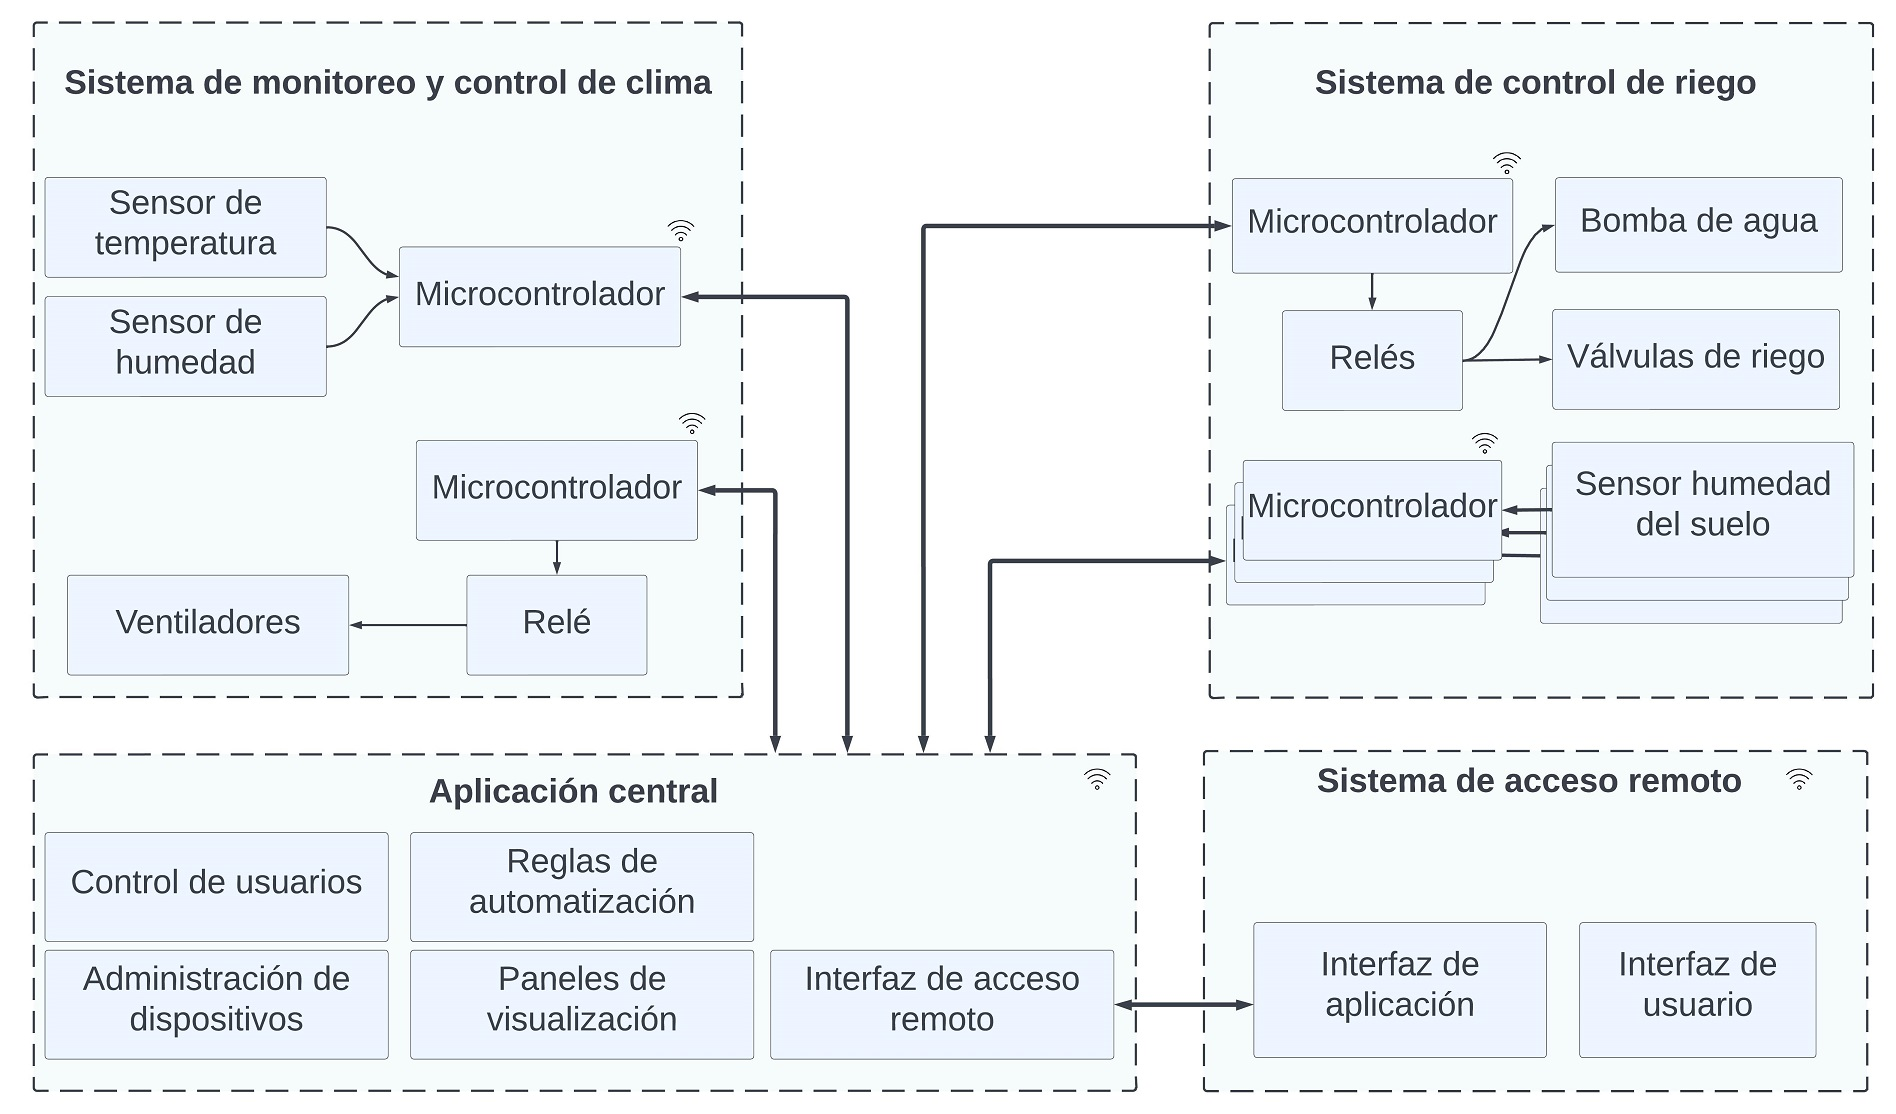
\includegraphics[width=1.0\textwidth]{./Figures/blockdiagram4.jpg}
	\caption[Arquitectura del sistema.]{Arquitectura del sistema.}
	\label{fig:blockdiagram}

\end{figure}


\subsection{Protocolos de comunicación}
\label{Protocolos de comunicación}
%\textit{Aquí se describe cómo se comunican los sistemas con la aplicación central y los protocolos usados en cada caso.}

%En la selección del software de la aplicación central se contempló la compatibilidad con múltiples protocolos de comunicación. Sin embargo limitaciones de configuración específicas, tal como el tiempo de retención de los mensajes en las colas de MQTT, forzaron el utilizar diferentes protocolos dependiendo del módulo en cuestión. Otro factor condicionante, como se detalla en la sección \ref{sec:Ciberseguridad del sistema}, fue el carecer de una CA que emita certificados que todos los componentes puedan confiar.

En esta sección se describe cómo se comunican los sistemas con la aplicación central y los protocolos usados en cada caso. En la figura \ref{fig:blockprotos} se aprecia un esquema simplificado que ilustra dichas interacciones.

Si bien tanto los módulos de hardware como el software soportan una gran variedad de protocolos,  se implementó MQTT en la mayoría de los casos conforme a los requerimientos. En algunas situaciones donde esto no fue técnicamente posible, se utilizó HTTP. Adicionalmente, para garantizar la seguridad de las comunicaciones, se incorporó un certificado autofirmado TLS en el servidor.

\begin{figure}[h]
	\centering
	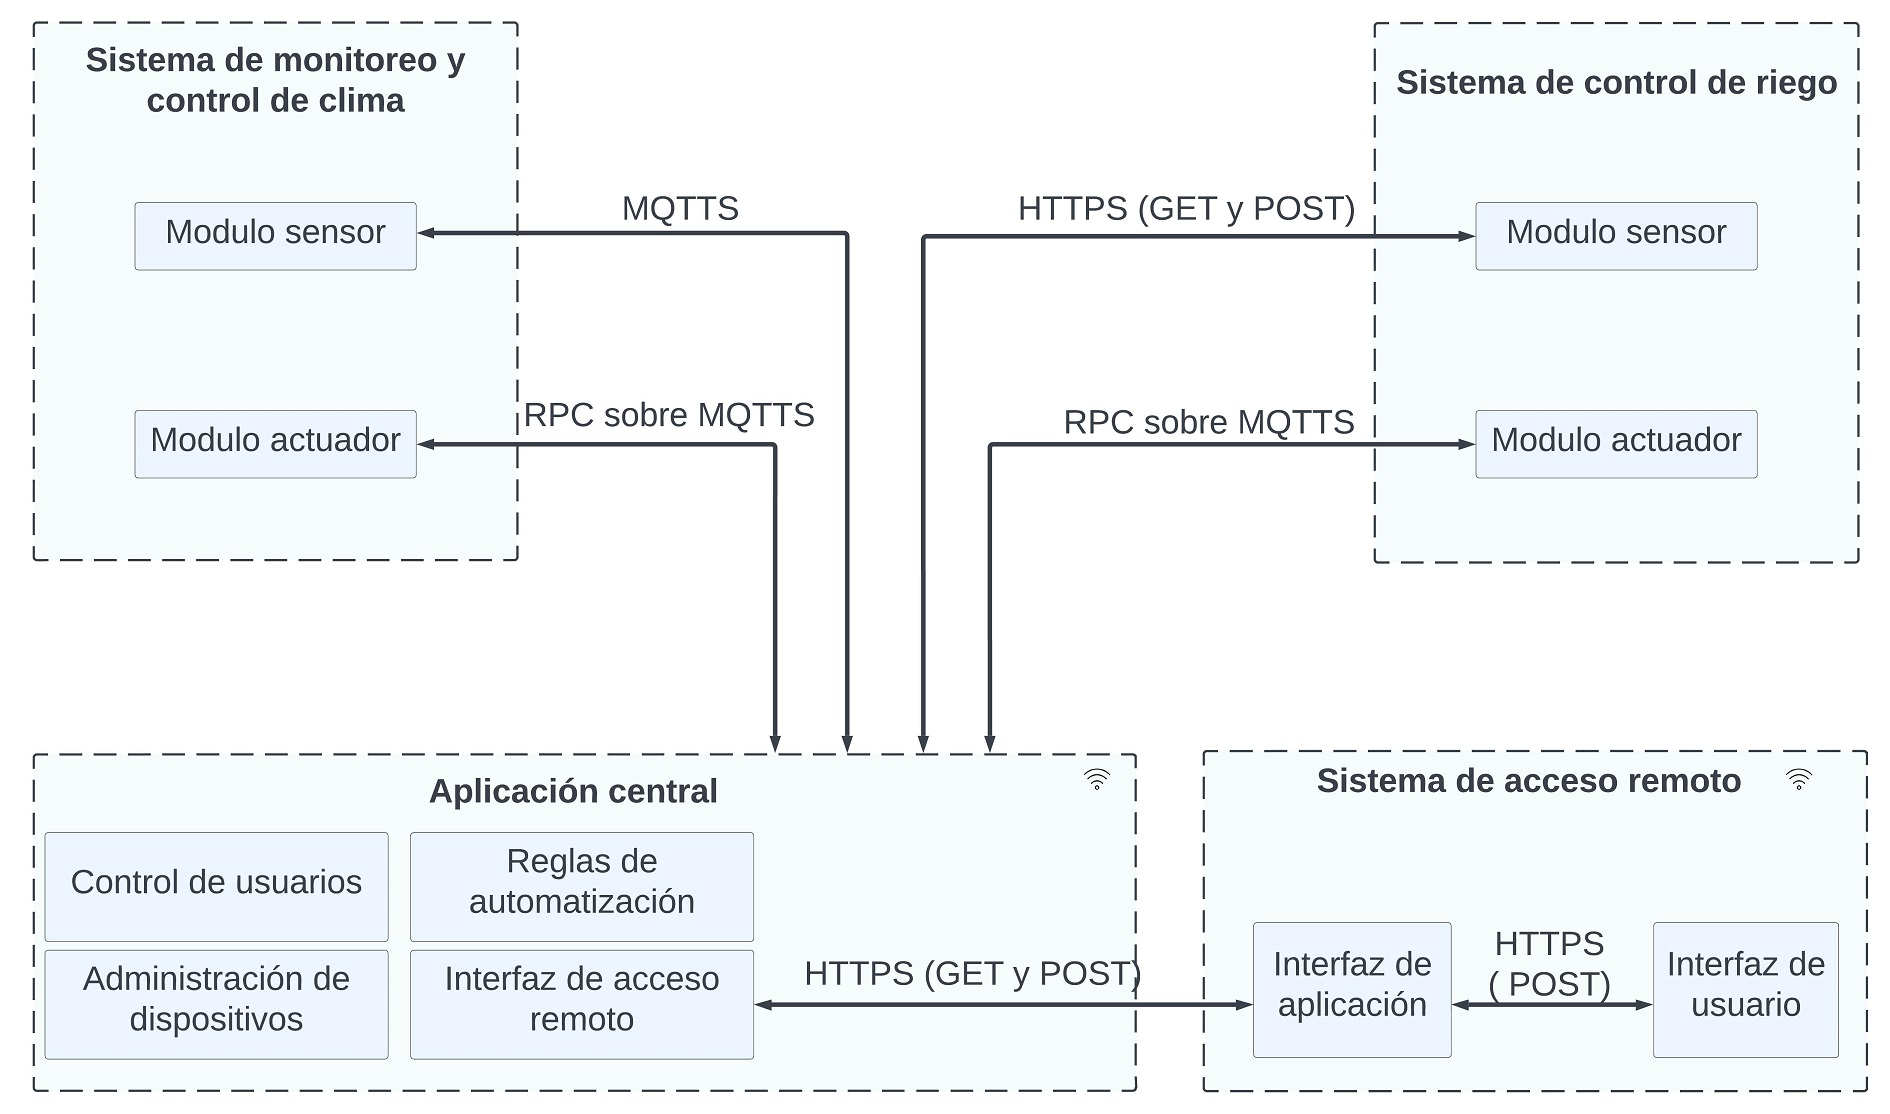
\includegraphics[width=1.0\textwidth]{./Figures/blockproto2.jpg}
	\caption[Protocolos de comunicación entre módulos.]{Protocolos de comunicación entre módulos.}
	\label{fig:blockprotos}
\end{figure}


\pagebreak
 A continuación se describen las interacciones principales entre los bloques componentes de la arquitectura:
 
 \begin{itemize}
	\item Sistema de monitoreo y control de clima: las comunicaciones desde y hasta este sistema son con la aplicación central.
	El módulo sensor envía las mediciones realizadas por medio de MQTT.
	En el caso que las variables del clima requieran una acción, la aplicación central comanda el encendido de los ventiladores por medio de un mensaje enviado por RPC \citep{rfc1057} sobre MQTT.
	
	\item Sistema de control de riego: las comunicaciones desde y hasta este sistema son con la aplicación central.
	El módulo sensor realiza dos conexiones, una para el envío de las mediciones y otra para recibir variables de configuración tales como el período de \textit{deep sleep}. Debido a limitaciones en la configuración de la persistencia de los mensajes en las colas de MQTT, se optó por utilizar llamadas HTTP (GET y POST) para realizar estas comunicaciones.
	Al igual que en el control de clima, la aplicación central inicia el riego por medio de mensajes RCP sobre MQTT hacia el controlador de la bomba y de las válvulas.
	
	\item Sistema de acceso remoto: la interfaz se comunica con la aplicación por medio de pedidos HTTP GET y POST para consultar el reporte de estado de los diferentes componentes. A continuación este se envia hacia la interfaz de usuario por medio de una solicitud HTTP POST.
 
 
 
 
 \end{itemize}






\section{Detalle de los módulos de hardware}
\label{sec:Módulos de hardware}
En esta sección se describen en detalle los esquemas de conexión de los distintos módulos y las consideraciones de diseño y construcción empleadas. 

\subsection{Módulos sensores de humedad del suelo}
\label{Módulos sensores de humedad del suelo}


En el proyecto se desarrollaron dos configuraciones diferentes de módulos para medir la humedad del suelo en macetas de diverso tipo y tamaño. Ambas opciones utilizan el microcontrolador ESP8266 pero incorporan un distinto número de sensores. En la figura \ref{fig:soilschem1} se muestra el esquema de conexión para la versión simple (con un único sensor) y en la figura \ref{fig:soilschem2} se ilustra la configuración doble.

Si bien en el prototipo los sensores se conectaron a una fuente de alimentación, la configuración y conexión del sistema está optimizada para el uso de baterías. Esto se debe a que los sensores pueden estar desplegados en múltiples ubicaciones dentro del invernadero y no siempre es posible conectarlos a la red eléctrica. 

El ahorro de energía necesario para permitir el uso de  baterías se logra a través de ciclos de apagado en los períodos donde no se realizan lecturas. A este mecanismo se lo que conoce como \textit{deep sleep} y una vez que el microcontrolador se encuentra en este estado se requiere un pulso eléctrico en el pin de \textit{reset} para que retorne al modo activo. 
Para habilitar la reactivación se interconectaron los pines D0 (GPIO16) y RST del chip ESP8266. En base a esta funcionalidad se logra una reducción del consumo de energía a valores muy pequeños que rondan los 0,3 mA durante el período de inactividad.




\begin{figure}[!h]
     \centering
     \begin{subfigure}[b]{0.45\textwidth}
		\centering
		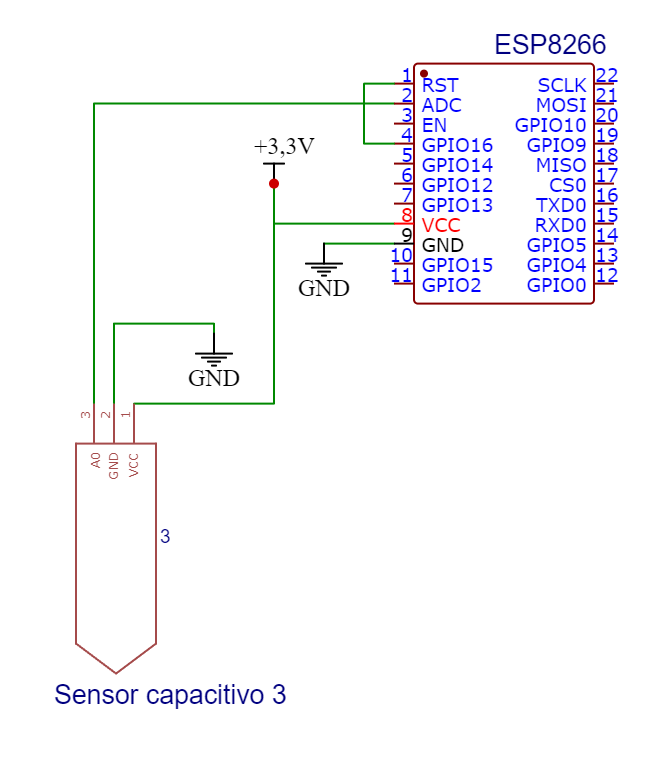
\includegraphics[width=0.9\textwidth]{./Figures/soil_schem_simple.png}
		\caption[Módulo sensor simple]{Módulo sensor simple.}
		\label{fig:soilschem1}
     \end{subfigure}
     \hfill
     \begin{subfigure}[b]{0.45\textwidth}
	\centering
		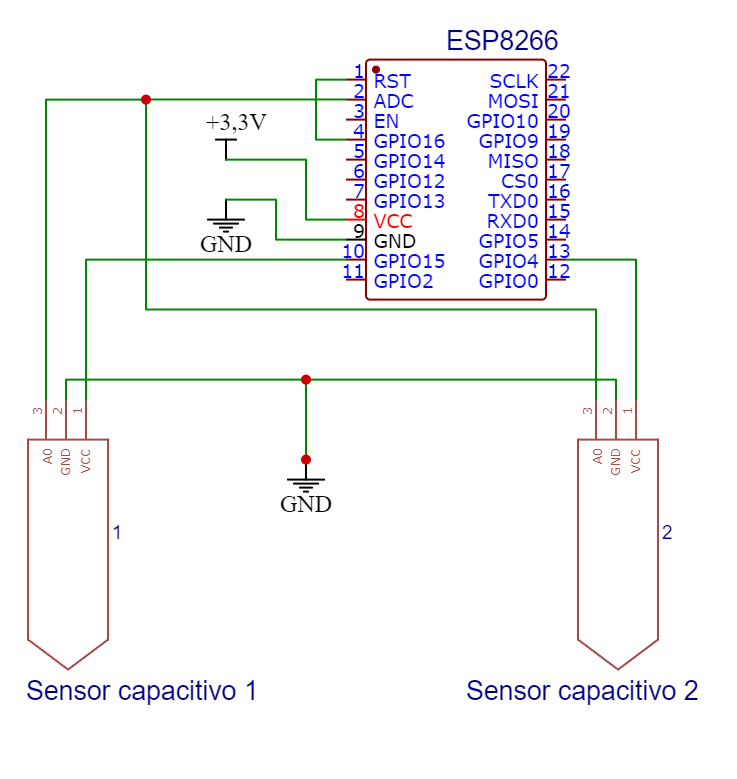
\includegraphics[width=1\textwidth]{./Figures/soil_schem_doble.png}
		\caption[Módulo sensor doble]{Módulo sensor doble.}
		\label{fig:soilschem2}
     \end{subfigure}
     \hfill
        \caption[Esquema de conexión de módulos sensores de humedad del suelo]{Esquema de conexión de módulos sensores de humedad del suelo.}	\label{fig:soilschem}
\end{figure}
%\begin{figure}[!h]
%	\centering
%	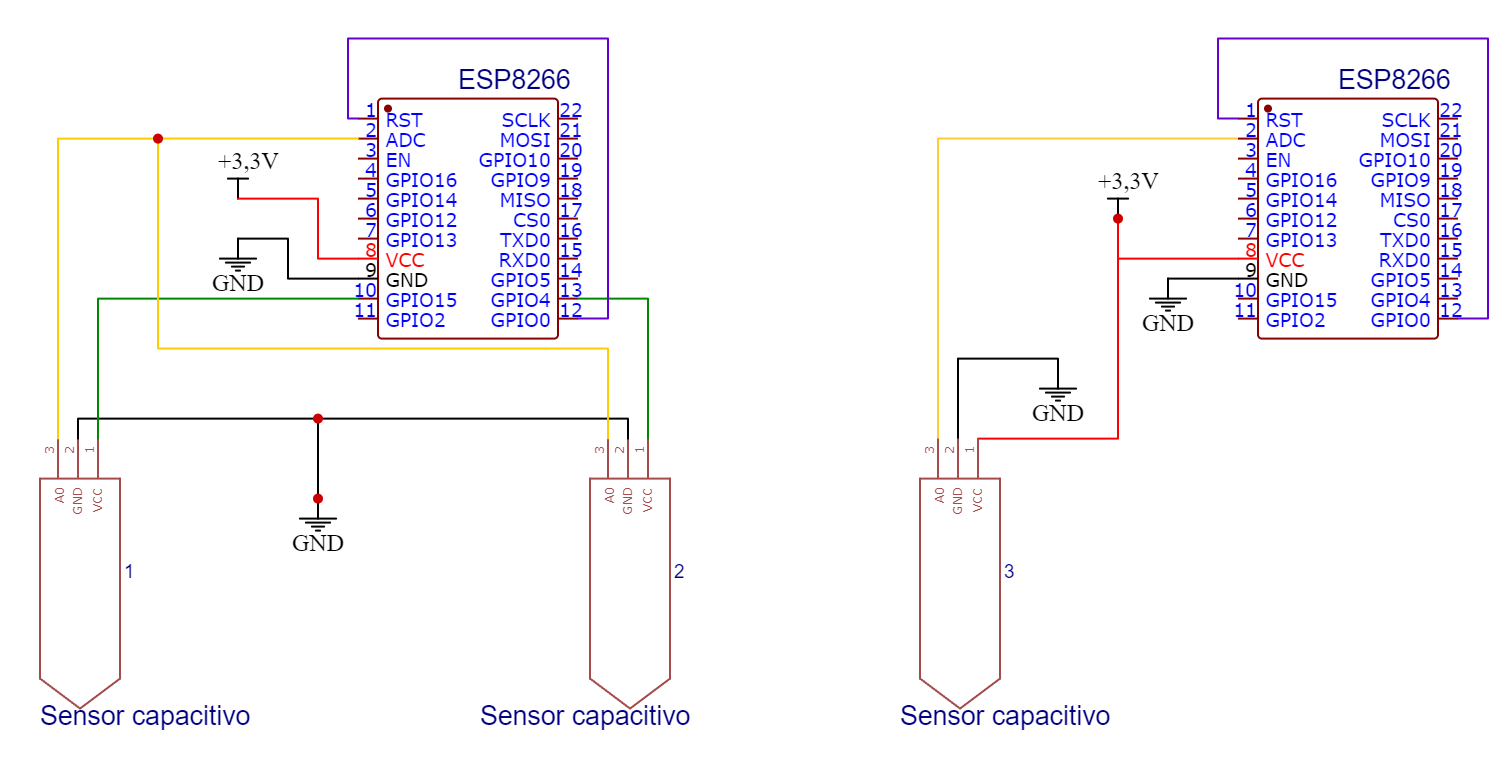
\includegraphics[width=1\textwidth]{./Figures/soil_schematic2.png}
%	\caption[Conexión del sensor de humedad del suelo]{Conexión del sensor de humedad del suelo.}
%	\label{fig:soilschem}
%\end{figure}

La integración de los componentes de los sensores se  realizó en forma manual por medio de placas de circuitos impresos (PCB) experimentales. En las figuras \ref{fig:soil1} y \ref{fig:soil2} se muestran los componentes empleados y un módulo ensamblado.

Dado que los sensores están expuestos a salpicaduras, se los recubrió con tubos adhesivos termocontraíbles que al aplicarles calor generan una protección a prueba de agua. Para el resguardo del chip ESP8266 se utilizó una caja de polipropileno transparente sellada. En las figuras \ref{fig:soil3} y \ref{fig:soil4} se muestran los componentes y sus protecciones. 

\begin{figure}[!h]
     \centering
     \begin{subfigure}[b]{0.45\textwidth}
		\centering
		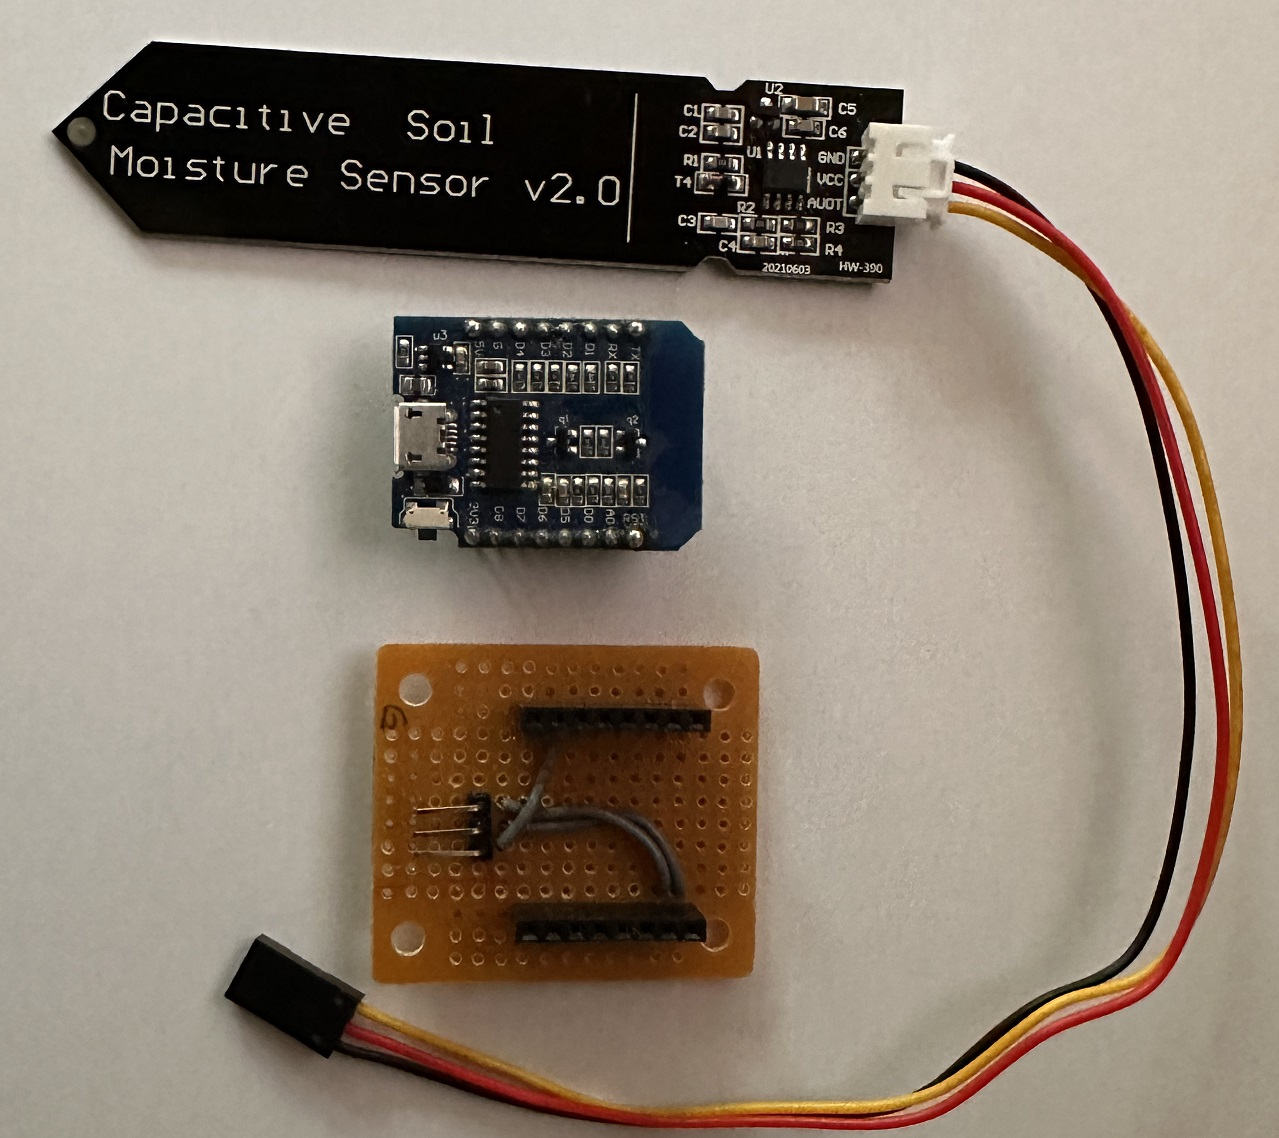
\includegraphics[width=0.60\textwidth]{./Figures/soil1.jpeg}
		\caption[Módulo con un sensor de humedad del suelo]{Módulo con un sensor de humedad del suelo.}
		\label{fig:soil1}
     \end{subfigure}
     \hfill
     \begin{subfigure}[b]{0.45\textwidth}
	\centering
		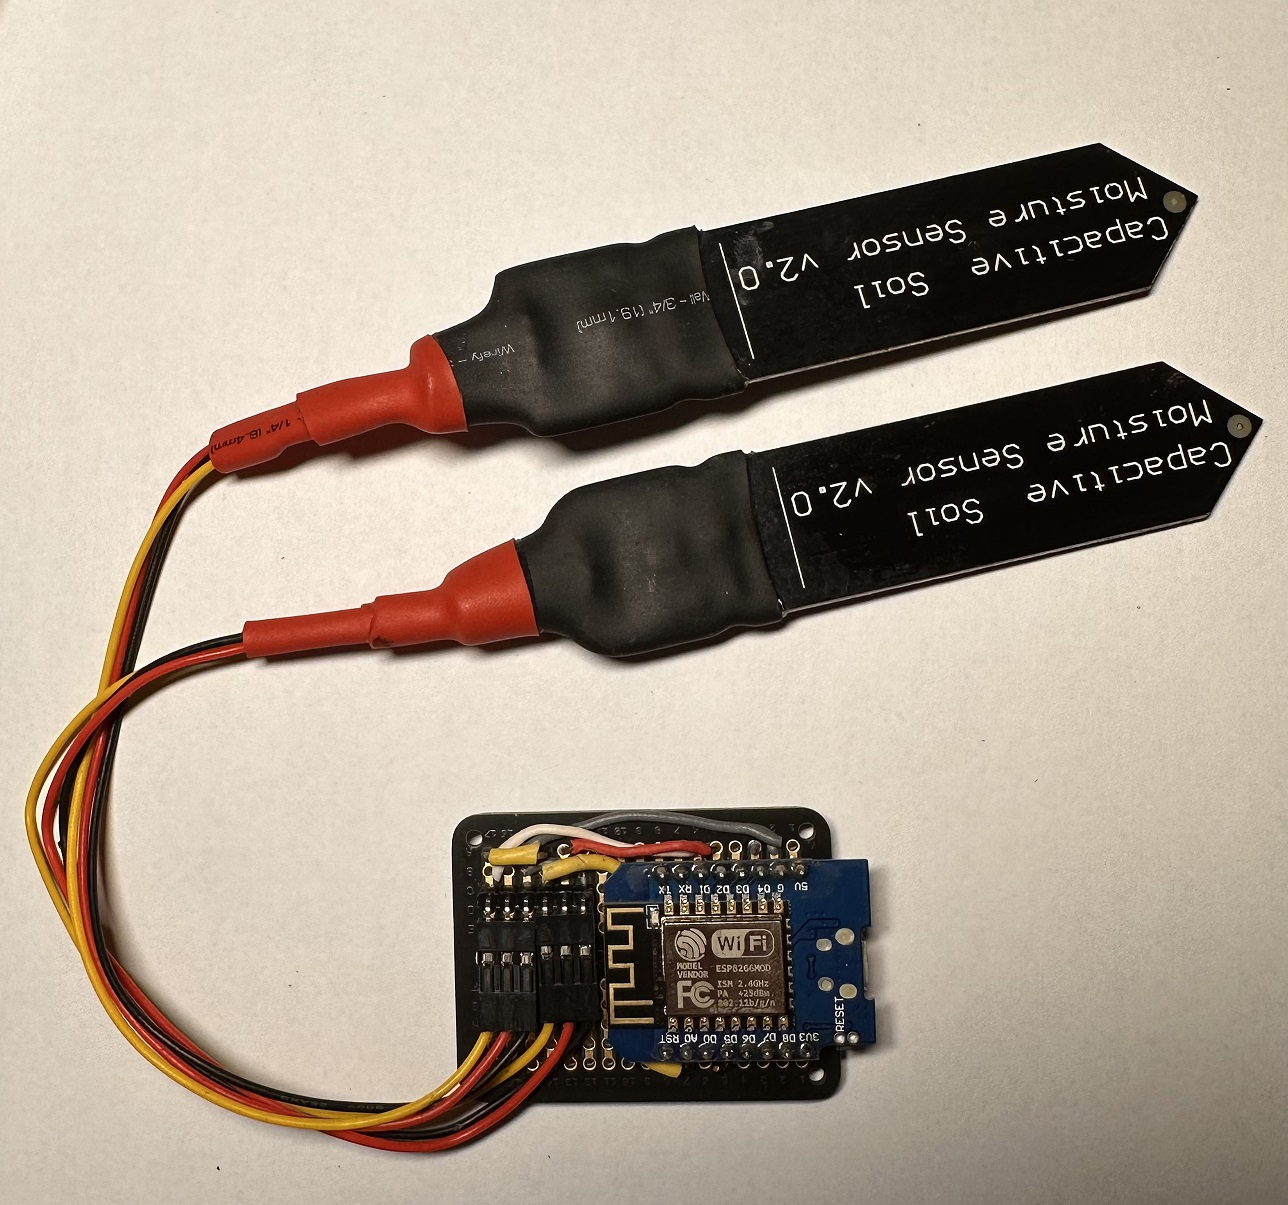
\includegraphics[width=0.60\textwidth]{./Figures/soil2.jpeg}
		\caption[Módulo con dos sensores de humedad del suelo]{Módulo con dos sensores de humedad del suelo.}
		\label{fig:soil2}
     \end{subfigure}
      \begin{subfigure}[b]{0.45\textwidth}
	\centering
		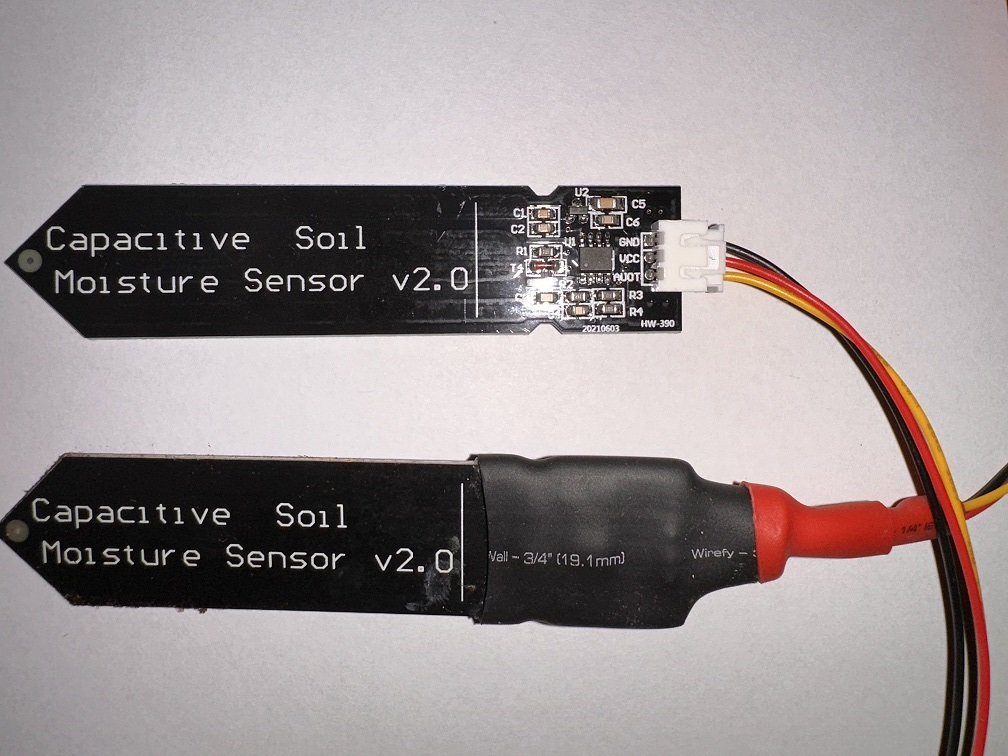
\includegraphics[width=0.60\textwidth]{./Figures/soil_compare.jpg}
		\caption[Detalle de protección de circuitos en los sensores]{Detalle de protección de circuitos en los sensores.}
		\label{fig:soil3}
     \end{subfigure}	
			\begin{subfigure}[b]{0.45\textwidth}
	\centering
		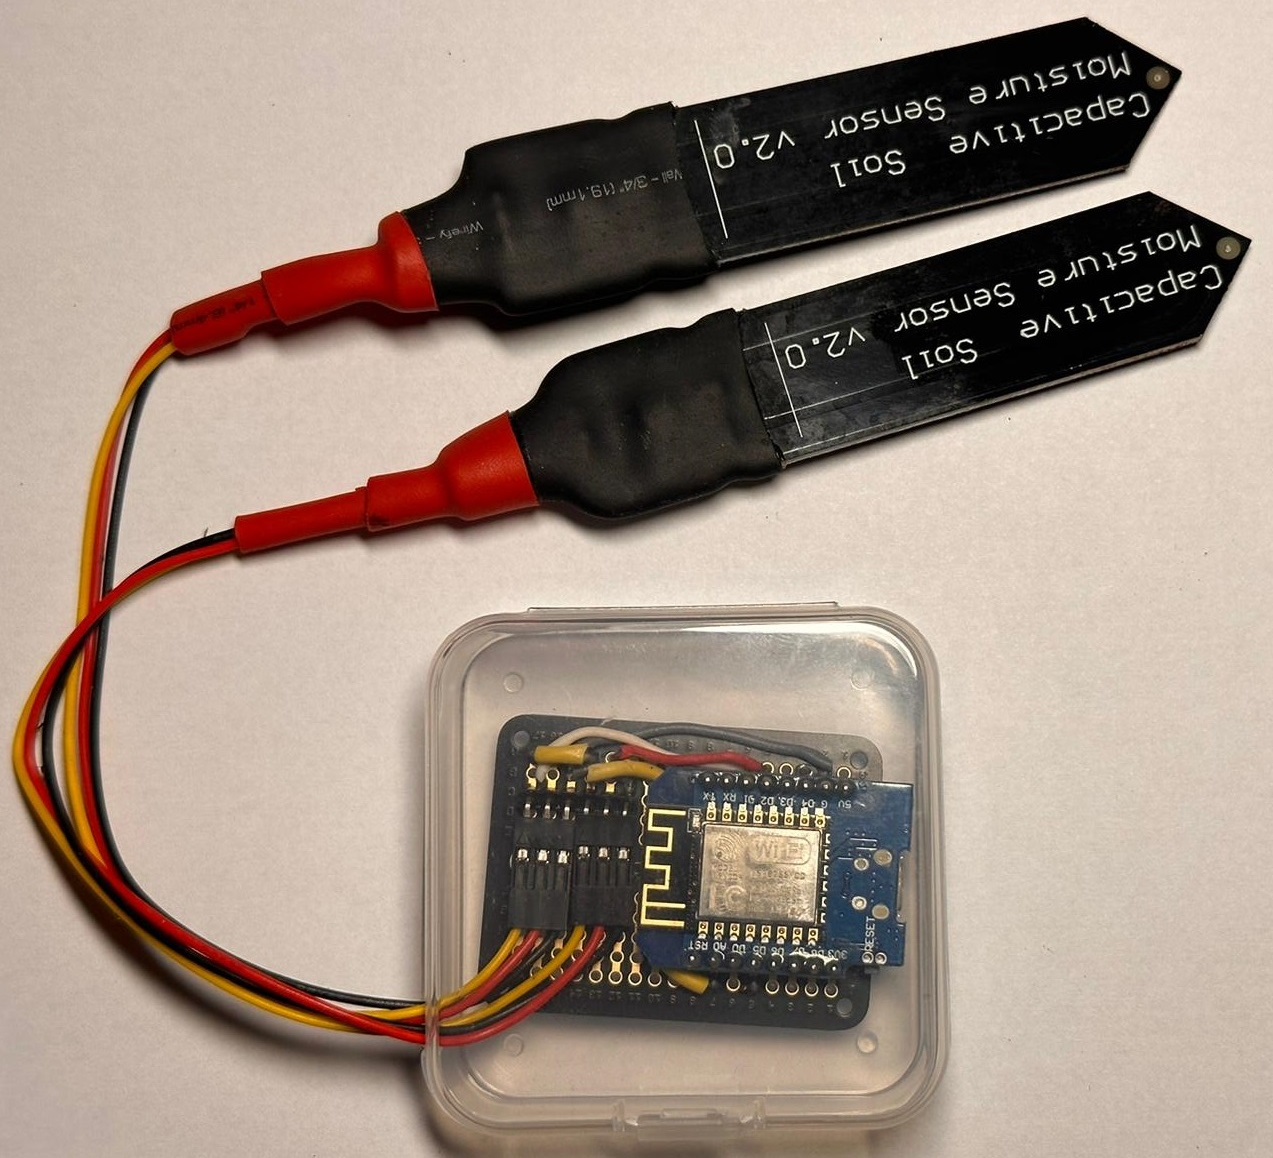
\includegraphics[width=0.60\textwidth]{./Figures/soil3.jpg}
		\caption[Módulo en su caja protectora]{Módulo en su caja protectora.}
		\label{fig:soil4}
     \end{subfigure}
     \hfill
        \caption[Módulos de sensores de humendad del suelo  empleados en el proyecto]{Módulo de sensores de humendad del suelo  empleados en el proyecto.}
        \label{fig:soilsenors}
\end{figure}


\pagebreak

\subsection{Módulo controlador del riego}
\label{Módulo controlador del riego}

Se compone de un microcontrolador ESP32, una placa de interfaz de relé de cuatro canales, un regulador DC-DC \textit{step down} de voltaje LM2596 y una pantalla LCD/OLED SSH1106. El esquema de conexiones entre estos componentes se detalla en la figura \ref{fig:riegochem}.

Todo el sistema (microcontrolador, bomba y válvulas de riego) se alimenta por medio de una fuente de 12 VDC. El regulador LM2596 reduce la tensión a 5 VDC para alimentar al chip ESP32, la pantalla y el circuito de control del relé.

Para la construcción del prototipo se realizó la integración del microcontrolador con la pantalla LCD mediante una placa PCB experimental. Tanto para el módulo regulador de tensión como para el conjunto de relés se emplearon circuitos preensamblados. En la figura \ref{fig:riego_control} se muestra todos los componentes ensamblados dentro de una caja protectora.   


\begin{figure}[!h]
	\centering
	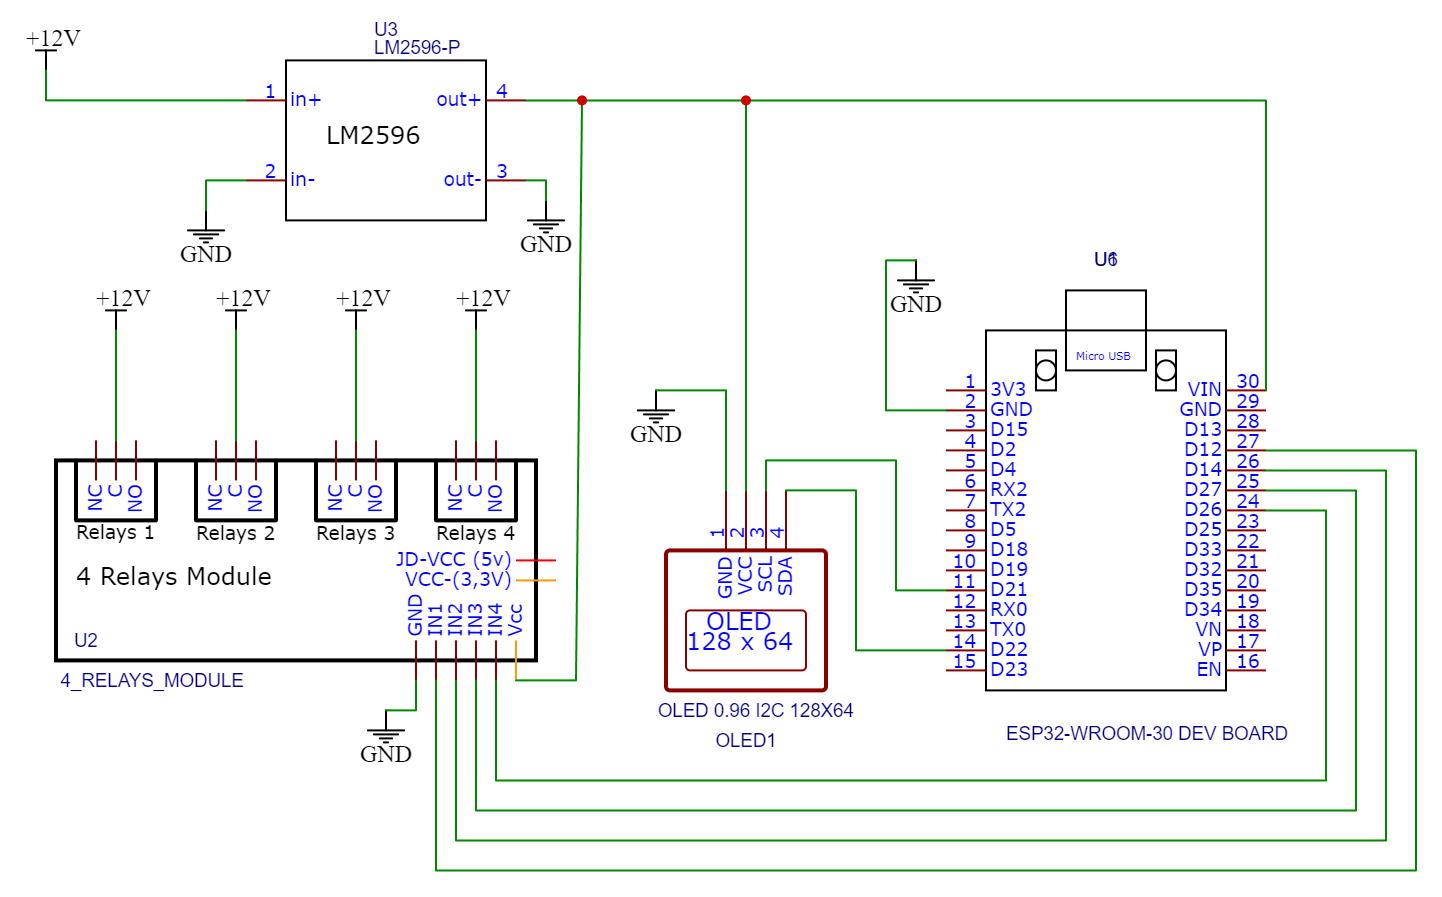
\includegraphics[width=0.9\textwidth]{./Figures/pump_schem.png}
	\caption[Conexión del módulo de control de riego]{Conexión del módulo de control de riego.}
	\label{fig:riegochem}
\end{figure}


Para el prototipo se construyó un módulo 





\begin{figure}[!h]
	\centering
	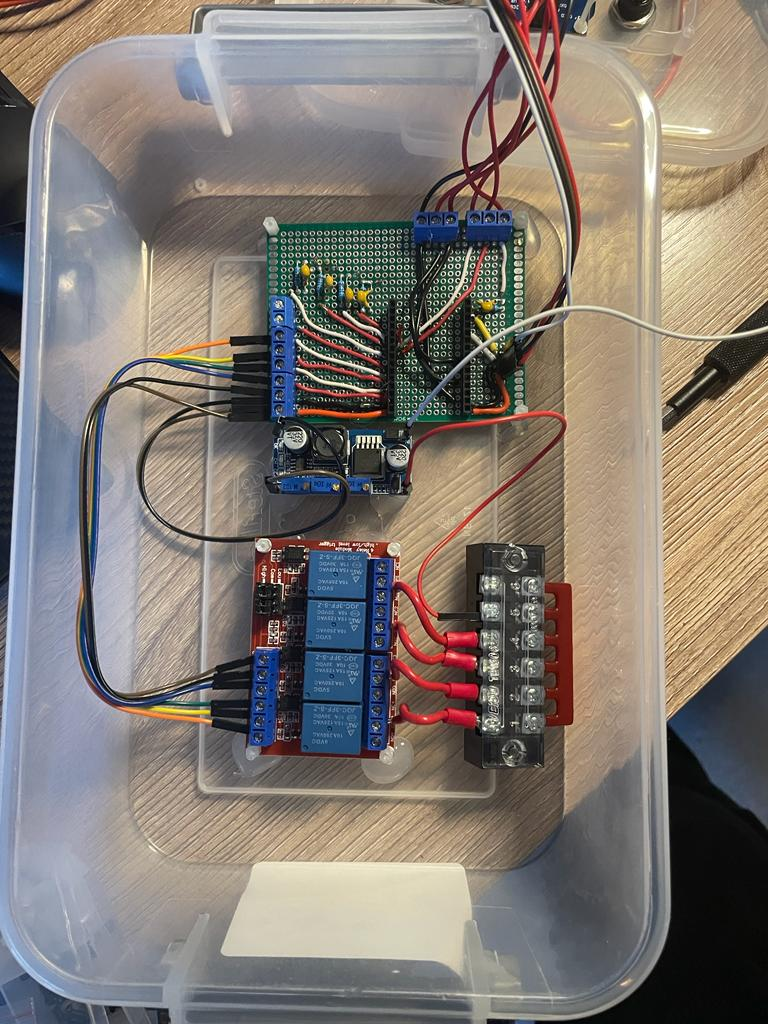
\includegraphics[width=0.5\textwidth]{./Figures/riego1.jpg}
	\caption[Modulo completo en su caja protectora]{Modulo completo en su caja protectora.}
	\label{fig:riego_control}
\end{figure}
 
\pagebreak

\subsection{Módulo sensor de temperatura y humedad}
\label{Módulo sensor de temperatura y humedad}

Está compuesto por un microcontrolador ESP8266, un sensor DHT22 y una pantalla LCD/OLED SSH1106 para visualizar los valores de temperatura y humedad  \textit{in situ} en tiempo real. El esquema de conexión de los componentes se puede ver en la figura \ref{fig:tempschem}.

A diferencia de los sensores de humedad del suelo, el sensor de temperatura y humedad está pensado para instalarse en forma permanente en un lugar determinado
con acceso a la red eléctrica. Por este motivo no se consideró necesario optimizar las conexiones para el uso de baterías.

%Dicha ubicación se elige de manera de lograr una medición representativa de las condiciones ambientales del invernadero. 

 

La construcción del módulo se realizó sobre placa PCB experimental en forma similar a los demás sistemas.
Para proteger los componentes se utilizó una caja de polipropileno transparente adaptada para permitir la entrada de alimentación y lograr que el sensor DHT22 quede expuesto al aire para medir las condiciones ambientales. 


\begin{figure}[!h]
	\centering
	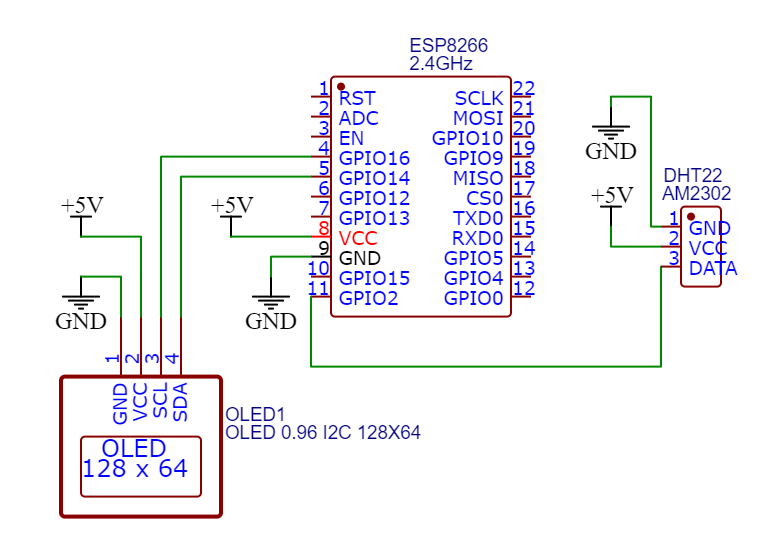
\includegraphics[width=0.7\textwidth]{./Figures/temp_sensor.png}
	\caption[Conexión del sensor de temperatura y humedad]{Conexión del sensor de temperatura y humedad
	.}
	\label{fig:tempschem}
\end{figure}


\begin{figure}[!h]
	\centering
	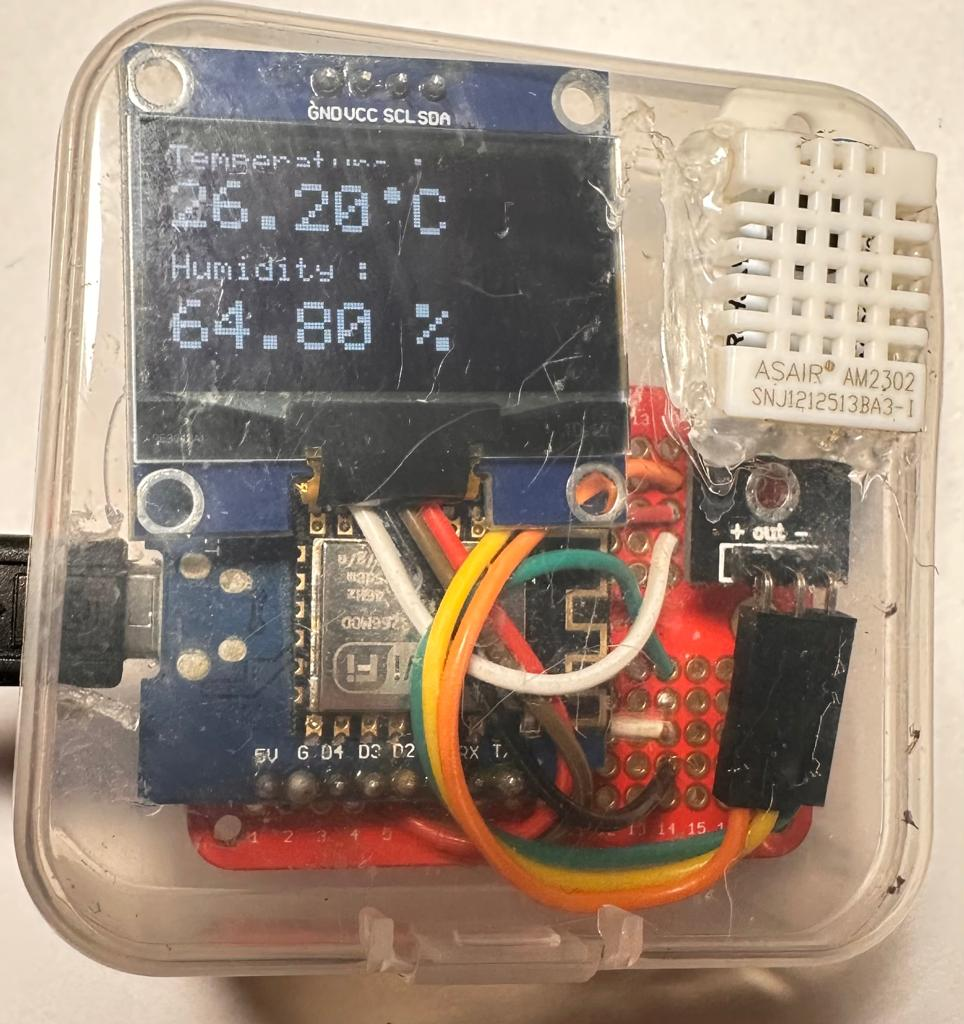
\includegraphics[width=0.5\textwidth]{./Figures/sensor_temp.jpg}
	\caption[Modulo completo en su caja protectora]{Modulo completo en su caja protectora.}
	\label{fig:temp_sensor}
\end{figure}

\pagebreak
\subsection{Módulo controlador de clima}
\label{Módulo controlador de clima}

Es el módulo responsable de accionar los ventiladores en el invernadero. Para el diseño se utilizó un chip ESP8266 conectado a un relé de una vía como se muestra en la figura \ref{fig:ventschem}. 

Dado que la salida del microcontrolador es de 3,3 V se seleccionó un relé que pueda ser accionado con ese valor de tensión, para evitar el uso de componentes adicionales tales como convertidores de tensión DC-DC \textit{step up}. 

En la figura\ref{fig:ventcontrol} ilustra el proceso de construcción del módulo. 



\begin{figure}[!h]
	\centering
	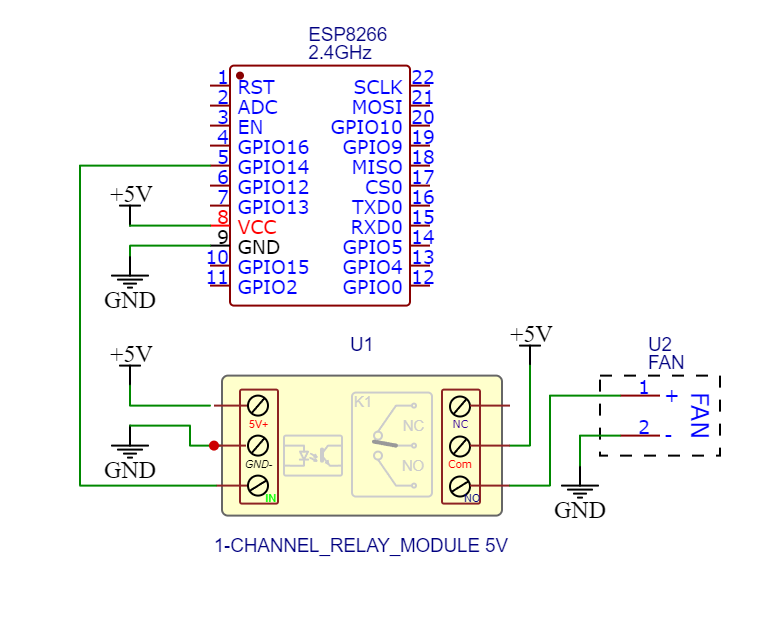
\includegraphics[width=0.7\textwidth]{./Figures/vent_schem.png}
	\caption[Conexión del modulo de control de clima]{Conexión del modulo de control de clima.}
	\label{fig:ventschem}
\end{figure}


\begin{figure}[!htpb]
     \centering
     \begin{subfigure}[b]{0.45\textwidth}
		\centering
		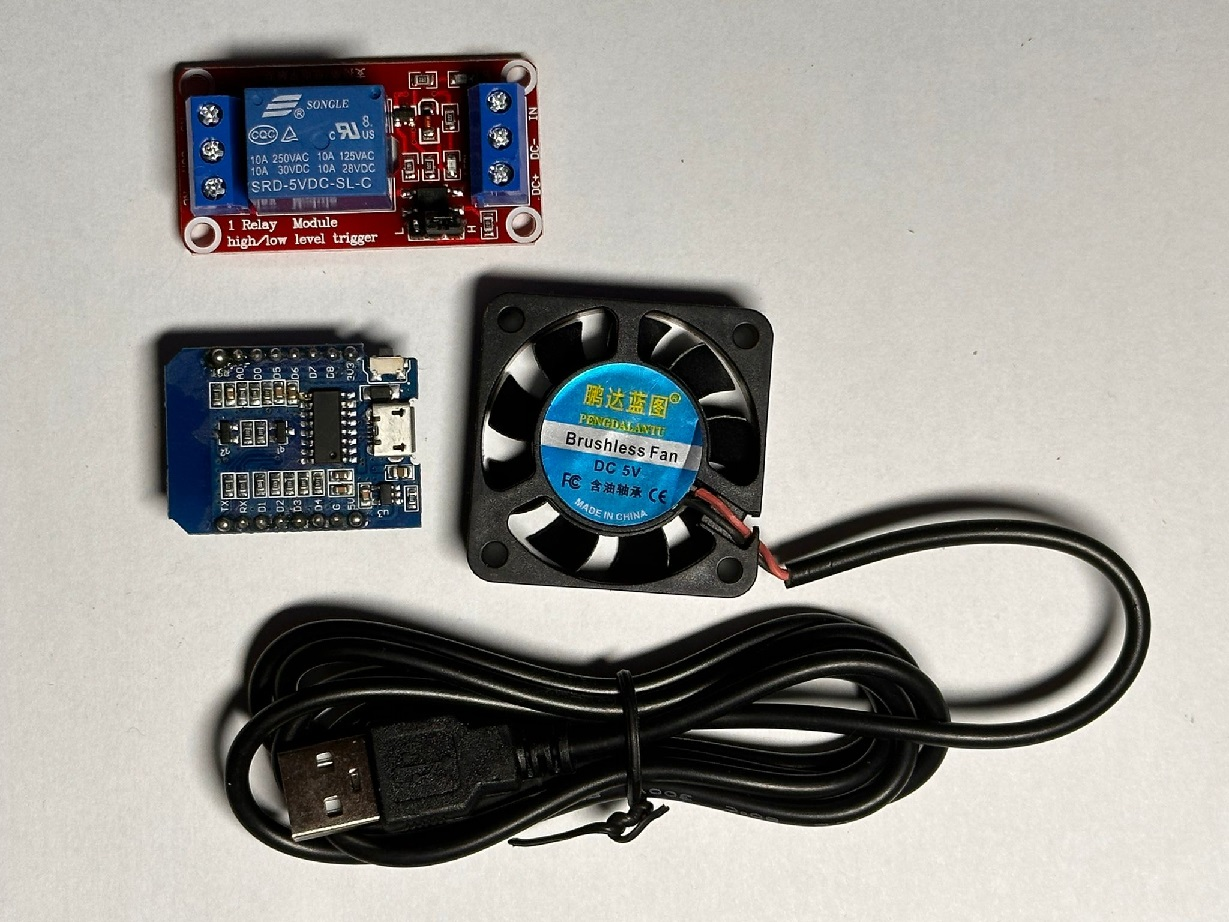
\includegraphics[width=0.80\textwidth]{./Figures/vent_control.jpg}
		\caption{Detalle de los componentes.}
		\label{fig:vent1}
     \end{subfigure}
     \hfill
     \begin{subfigure}[b]{0.45\textwidth}
	\centering
		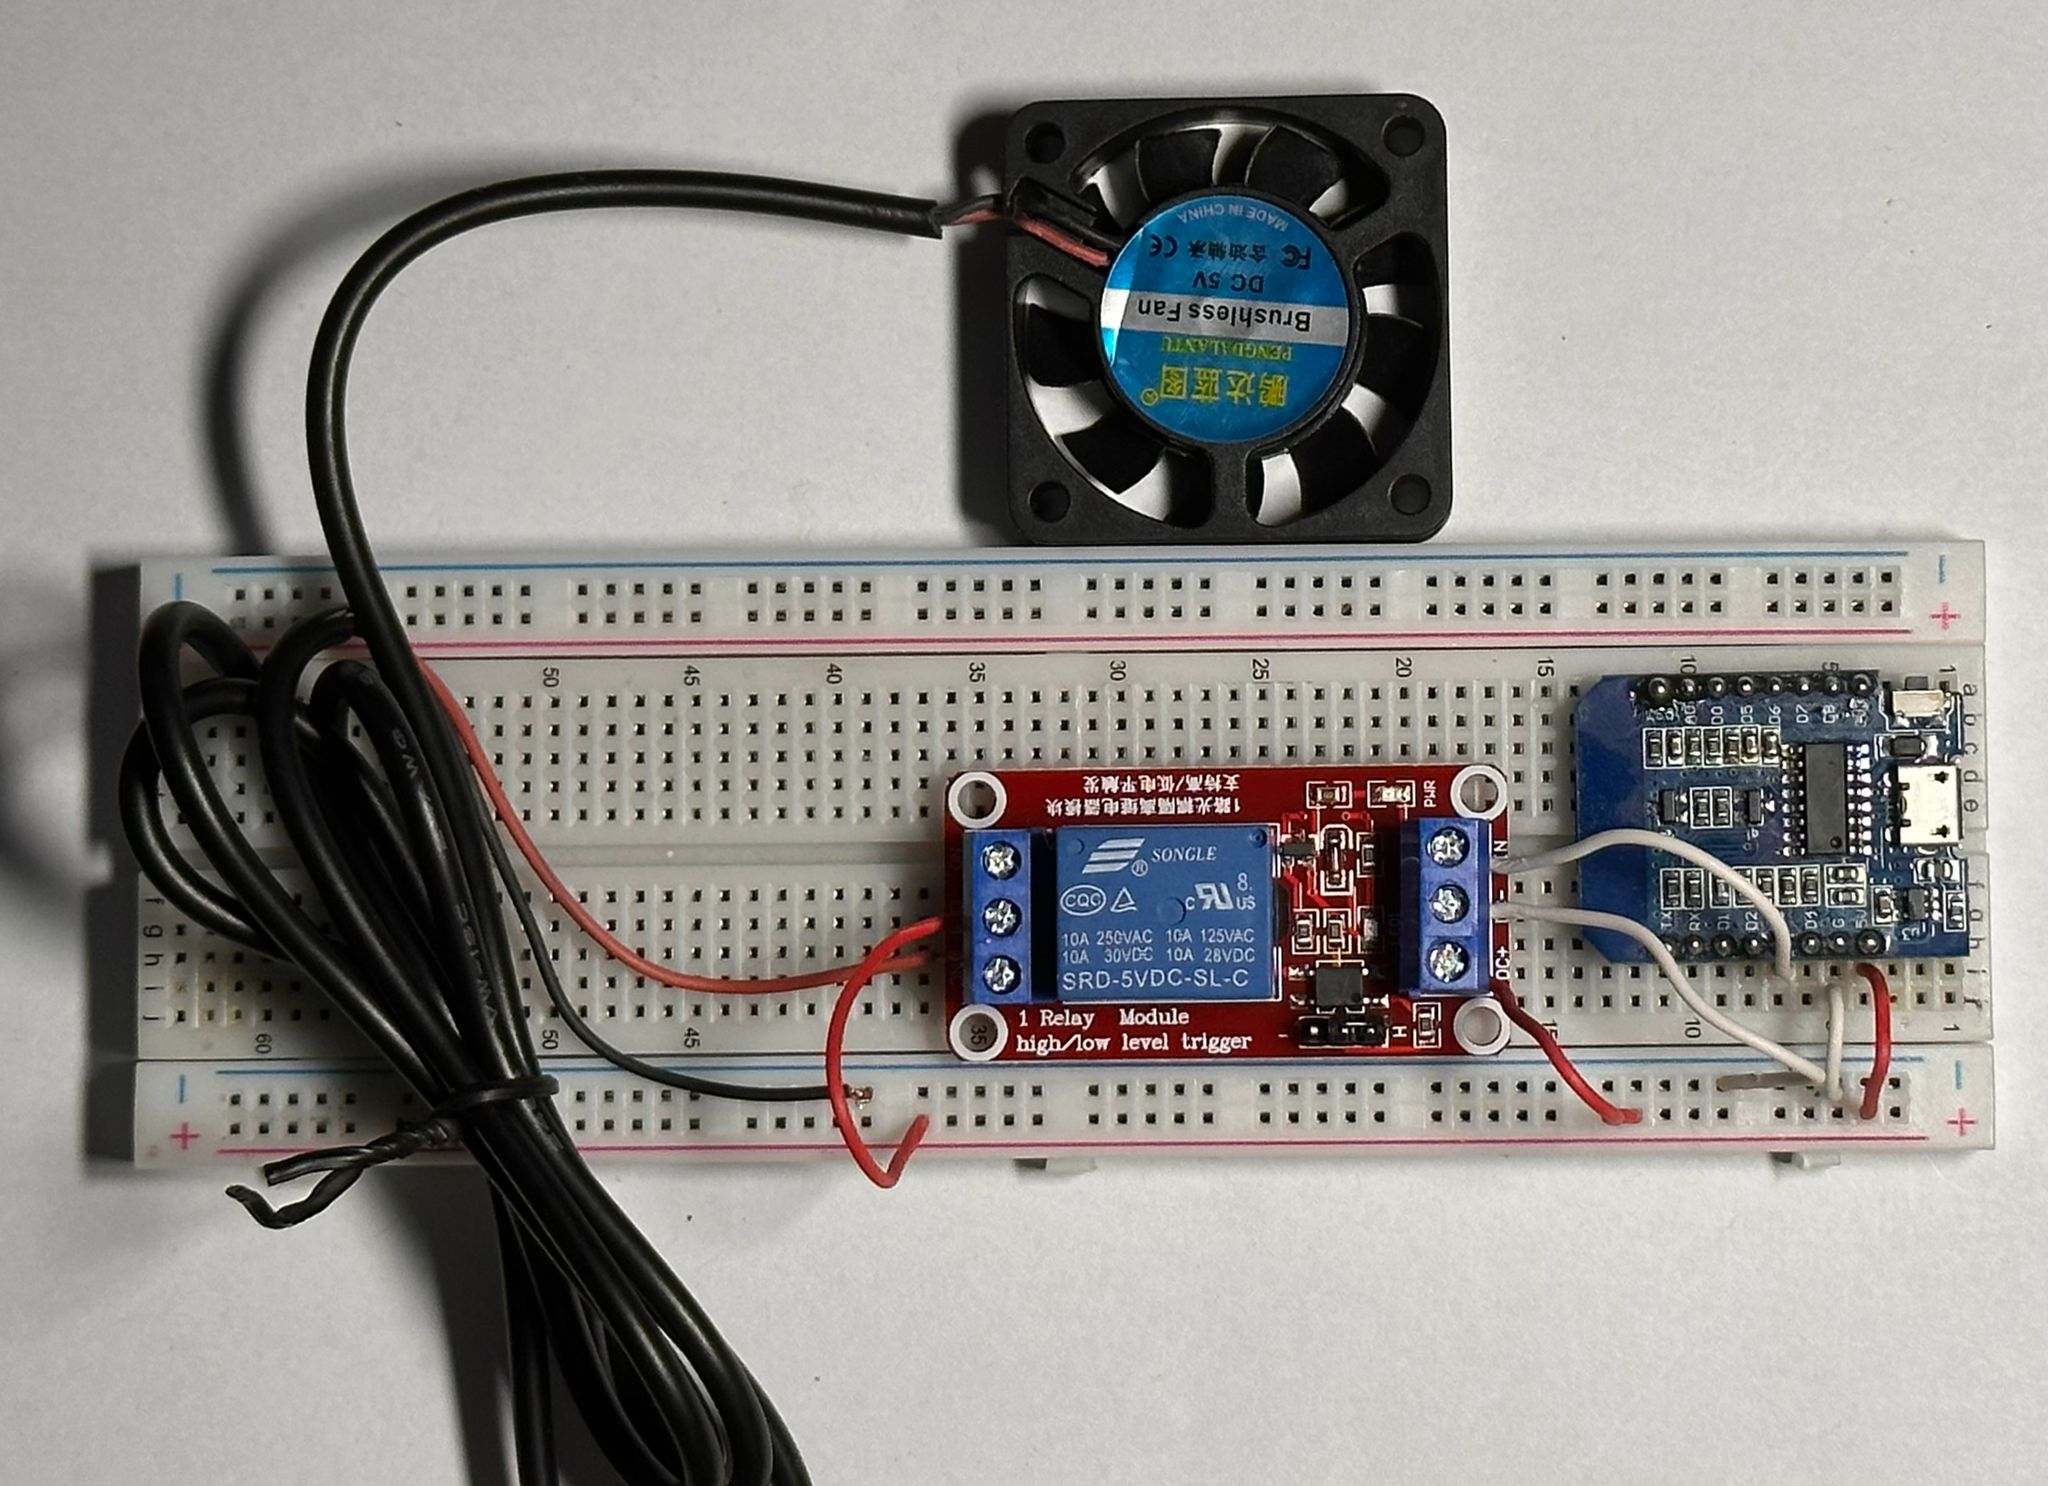
\includegraphics[width=0.80\textwidth]{./Figures/vent_proto.jpg}
		\caption{Configuración del módulo.}
		\label{fig:vent2}
     \end{subfigure}	
	\begin{subfigure}[b]{0.45\textwidth}
		\centering
		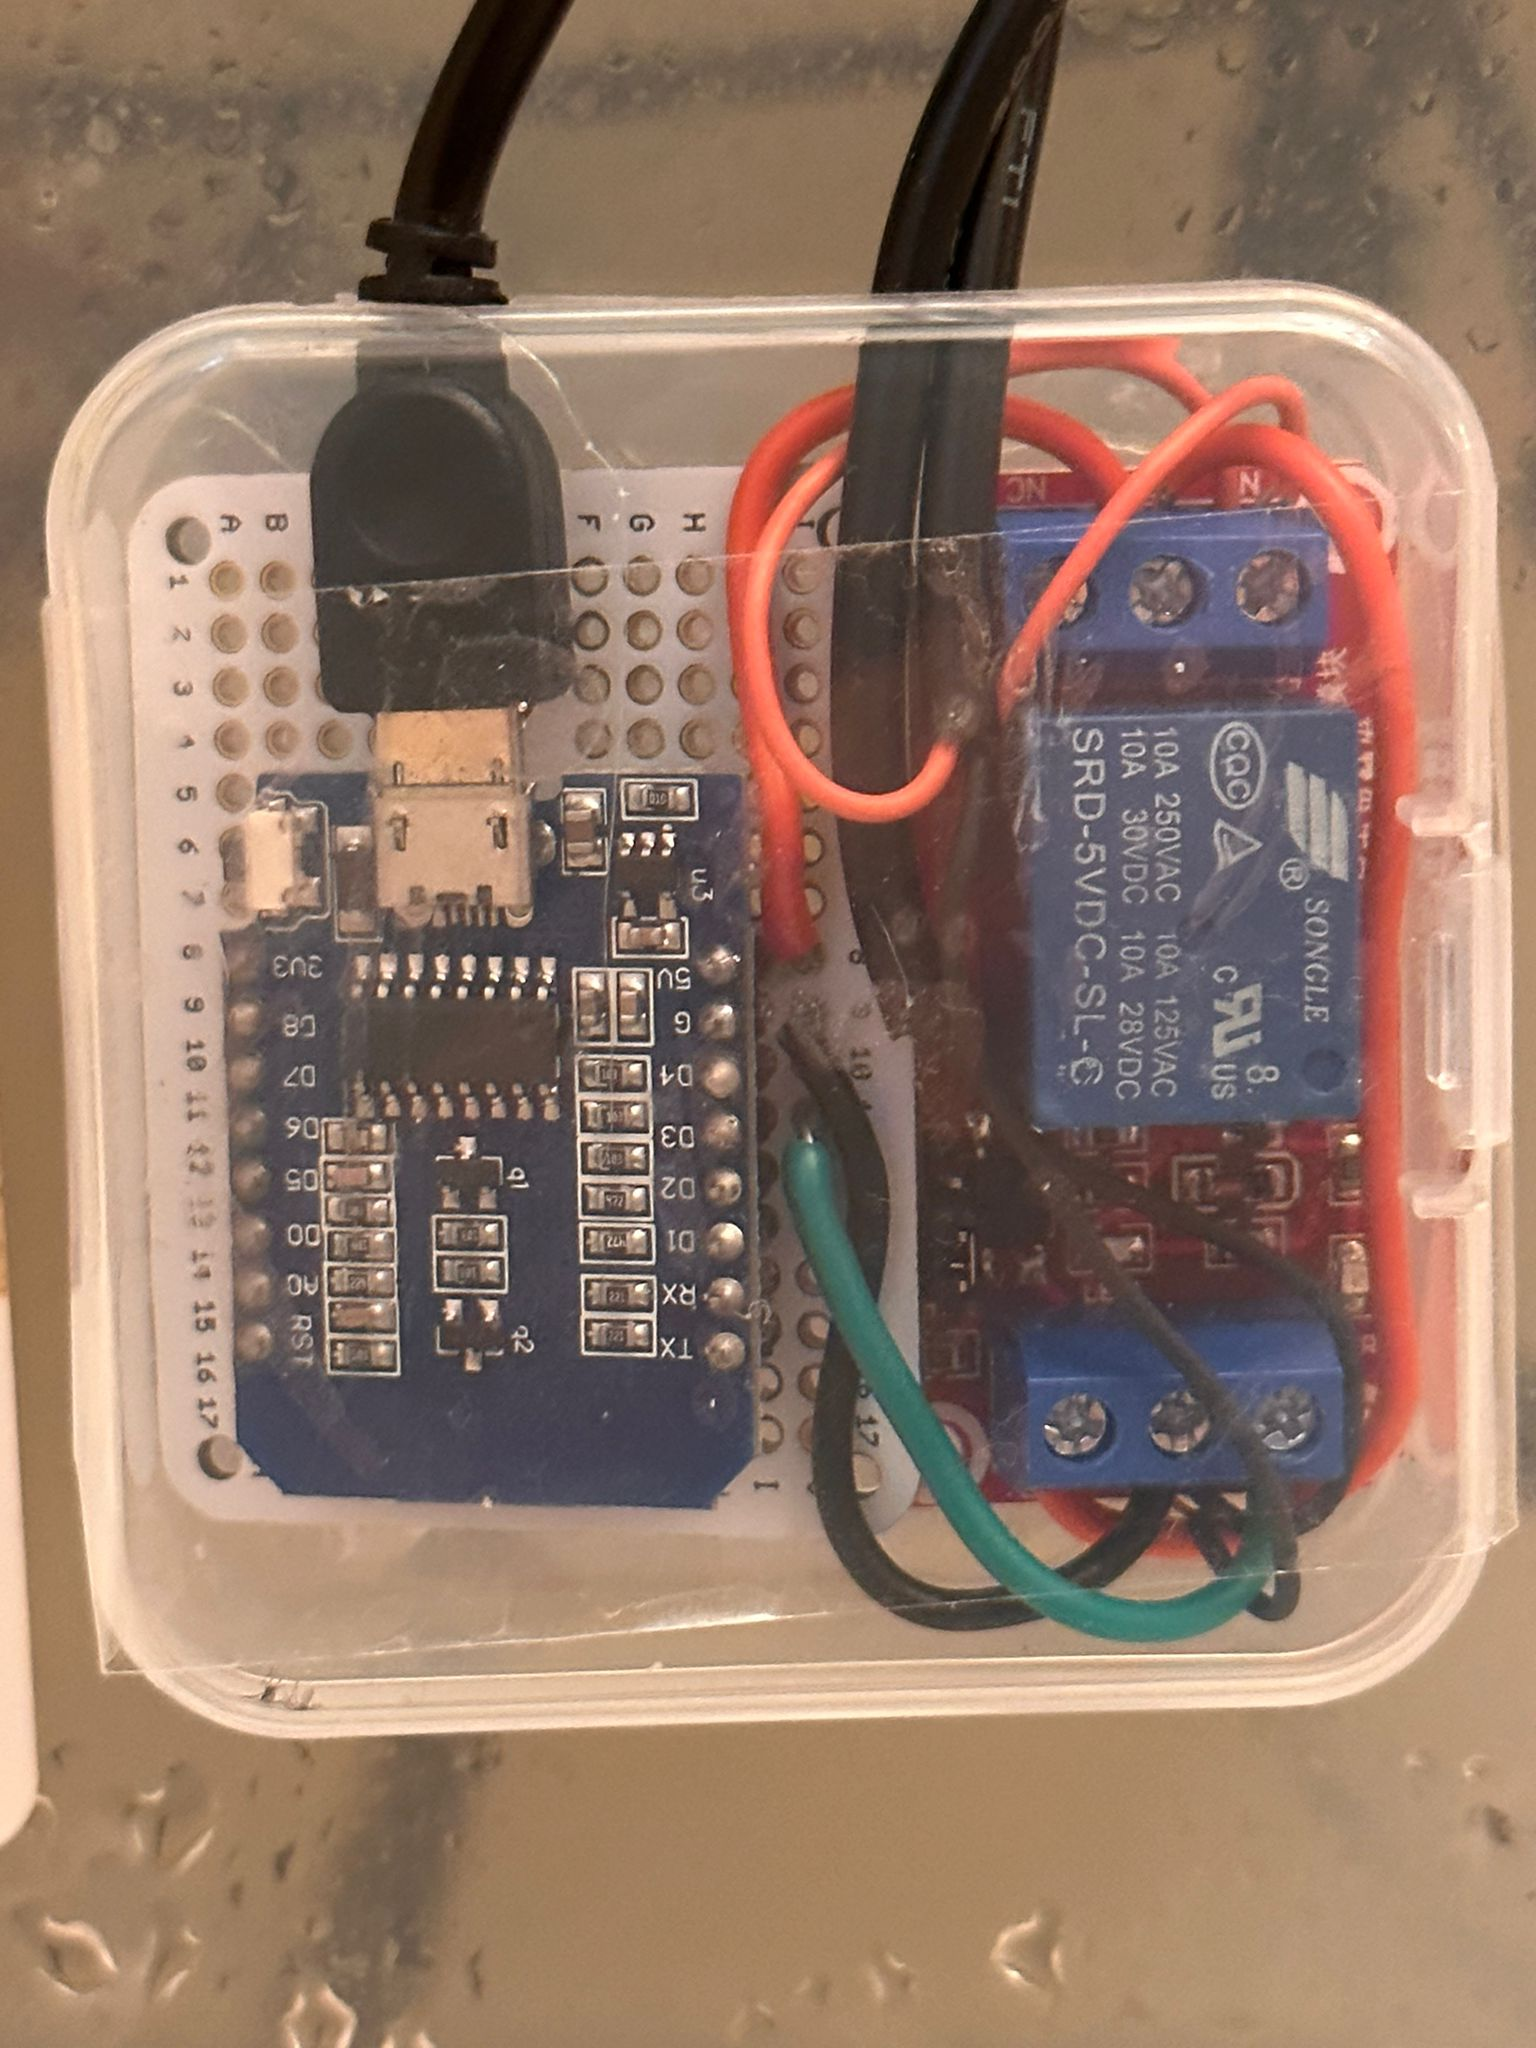
\includegraphics[width=0.60\textwidth]{./Figures/vent_assembled.jpg}
		\caption{Módulo finalizado en su caja protectora.}
		\label{fig:vent3}
     \end{subfigure}
     \hfill
        \caption[Módulo de control del clima]{Módulo de control del clima.}
        \label{fig:ventcontrol}
\end{figure}


\pagebreak

\section{Detalle del firmware desarrollado}
\label{sec:Desarrollo del firmware}


%\subsection{Programación del microcontrolador de medición de clima}
%\label{Programación del microcontrolador de medición de clima}


\section{Selección y configuración del software}
\label{sec:Selección y configuración del software}

\section{Ciberseguridad del sistema}
\label{sec:Ciberseguridad del sistema}
